% Options for packages loaded elsewhere
\PassOptionsToPackage{unicode}{hyperref}
\PassOptionsToPackage{hyphens}{url}
\PassOptionsToPackage{dvipsnames,svgnames,x11names}{xcolor}
%
\documentclass[
  11pt,
]{article}
\usepackage{amsmath,amssymb}
\usepackage{iftex}
\ifPDFTeX
  \usepackage[T1]{fontenc}
  \usepackage[utf8]{inputenc}
  \usepackage{textcomp} % provide euro and other symbols
\else % if luatex or xetex
  \usepackage{unicode-math} % this also loads fontspec
  \defaultfontfeatures{Scale=MatchLowercase}
  \defaultfontfeatures[\rmfamily]{Ligatures=TeX,Scale=1}
\fi
\usepackage{lmodern}
\ifPDFTeX\else
  % xetex/luatex font selection
\fi
% Use upquote if available, for straight quotes in verbatim environments
\IfFileExists{upquote.sty}{\usepackage{upquote}}{}
\IfFileExists{microtype.sty}{% use microtype if available
  \usepackage[]{microtype}
  \UseMicrotypeSet[protrusion]{basicmath} % disable protrusion for tt fonts
}{}
\makeatletter
\@ifundefined{KOMAClassName}{% if non-KOMA class
  \IfFileExists{parskip.sty}{%
    \usepackage{parskip}
  }{% else
    \setlength{\parindent}{0pt}
    \setlength{\parskip}{6pt plus 2pt minus 1pt}}
}{% if KOMA class
  \KOMAoptions{parskip=half}}
\makeatother
\usepackage{xcolor}
\usepackage[margin=0.85in]{geometry}
\usepackage{longtable,booktabs,array}
\usepackage{calc} % for calculating minipage widths
% Correct order of tables after \paragraph or \subparagraph
\usepackage{etoolbox}
\makeatletter
\patchcmd\longtable{\par}{\if@noskipsec\mbox{}\fi\par}{}{}
\makeatother
% Allow footnotes in longtable head/foot
\IfFileExists{footnotehyper.sty}{\usepackage{footnotehyper}}{\usepackage{footnote}}
\makesavenoteenv{longtable}
\usepackage{graphicx}
\makeatletter
\def\maxwidth{\ifdim\Gin@nat@width>\linewidth\linewidth\else\Gin@nat@width\fi}
\def\maxheight{\ifdim\Gin@nat@height>\textheight\textheight\else\Gin@nat@height\fi}
\makeatother
% Scale images if necessary, so that they will not overflow the page
% margins by default, and it is still possible to overwrite the defaults
% using explicit options in \includegraphics[width, height, ...]{}
\setkeys{Gin}{width=\maxwidth,height=\maxheight,keepaspectratio}
% Set default figure placement to htbp
\makeatletter
\def\fps@figure{htbp}
\makeatother
\setlength{\emergencystretch}{3em} % prevent overfull lines
\providecommand{\tightlist}{%
  \setlength{\itemsep}{0pt}\setlength{\parskip}{0pt}}
\setcounter{secnumdepth}{-\maxdimen} % remove section numbering
% definitions for citeproc citations
\NewDocumentCommand\citeproctext{}{}
\NewDocumentCommand\citeproc{mm}{%
  \begingroup\def\citeproctext{#2}\cite{#1}\endgroup}
\makeatletter
 % allow citations to break across lines
 \let\@cite@ofmt\@firstofone
 % avoid brackets around text for \cite:
 \def\@biblabel#1{}
 \def\@cite#1#2{{#1\if@tempswa , #2\fi}}
\makeatother
\newlength{\cslhangindent}
\setlength{\cslhangindent}{1.5em}
\newlength{\csllabelwidth}
\setlength{\csllabelwidth}{3em}
\newenvironment{CSLReferences}[2] % #1 hanging-indent, #2 entry-spacing
 {\begin{list}{}{%
  \setlength{\itemindent}{0pt}
  \setlength{\leftmargin}{0pt}
  \setlength{\parsep}{0pt}
  % turn on hanging indent if param 1 is 1
  \ifodd #1
   \setlength{\leftmargin}{\cslhangindent}
   \setlength{\itemindent}{-1\cslhangindent}
  \fi
  % set entry spacing
  \setlength{\itemsep}{#2\baselineskip}}}
 {\end{list}}
\usepackage{calc}
\newcommand{\CSLBlock}[1]{\hfill\break\parbox[t]{\linewidth}{\strut\ignorespaces#1\strut}}
\newcommand{\CSLLeftMargin}[1]{\parbox[t]{\csllabelwidth}{\strut#1\strut}}
\newcommand{\CSLRightInline}[1]{\parbox[t]{\linewidth - \csllabelwidth}{\strut#1\strut}}
\newcommand{\CSLIndent}[1]{\hspace{\cslhangindent}#1}
\ifLuaTeX
\usepackage[bidi=basic]{babel}
\else
\usepackage[bidi=default]{babel}
\fi
\babelprovide[main,import]{british}
% get rid of language-specific shorthands (see #6817):
\let\LanguageShortHands\languageshorthands
\def\languageshorthands#1{}
\ifLuaTeX
  \usepackage{selnolig}  % disable illegal ligatures
\fi
\usepackage{bookmark}
\IfFileExists{xurl.sty}{\usepackage{xurl}}{} % add URL line breaks if available
\urlstyle{same}
\hypersetup{
  pdftitle={A Controlled Evaluation of Graph Conditioned Evidence Weighting for Gene Regulatory Network Inference},
  pdflang={en-GB},
  colorlinks=true,
  linkcolor={black},
  filecolor={Maroon},
  citecolor={Blue},
  urlcolor={blue},
  pdfcreator={LaTeX via pandoc}}

\title{A Controlled Evaluation of Graph Conditioned Evidence Weighting
for Gene Regulatory Network Inference}
\author{}
\date{28 November 2026}

\begin{document}
\maketitle

\section{Abstract}\label{abstract}

Biological priors can assist gene regulatory network inference, but
their usefulness depends on how evidence changes an inference decision.
We evaluated graph-conditional evidence valuation (GCEV), a one-step
procedure that learns source weights from nested, paired comparisons of
graph edits with and without an evidence source. Target-held-out
learning separates the utility observations for a gene from the model
predicting its weights. Three prospectively locked simulation studies
used 48, 32 and 32 independently seeded directed acyclic networks to
test graph-state information, a nonlinear-interaction hypothesis and an
explicit parent-feature ablation. In the 48-network primary comparison,
the estimated GCEV-minus-control average-precision difference was
0.007715, with a 95\% network-bootstrap interval of −0.010750 to
0.026722. Fixed weighting exceeded GCEV by 0.074505 average precision on
clean evidence. Neither subsequent study met its primary success
criterion. A developmental K562 comparison used 394 fitting cells, 131
evaluation cells, 16 transcription factors, 64 genes, sequence-motif
priors and DNase accessibility. The primary
GCEV-minus-source-feature-only prediction-error difference was
−0.000223, with a conditional paired-cell interval of −0.000636 to
0.000175. Accessibility represented as an additive target-constant term
could not alter within-target transcription-factor selection, despite
positive learned accessibility weights for 47 of 64 targets.
Multiplicative representations changed decisions, but their predictive
usefulness was not evaluated. These results do not establish an
advantage for the tested graph-state representation. They identify a
distinction between evidence availability, influence on an action and
observed predictive utility, while delimiting the conclusions supported
by small simulations and a single real-data cohort.

\textbf{Keywords:} gene regulatory network inference; biological priors;
adaptive evidence weighting; graph-state features; controlled
evaluation; source utility; single-cell transcriptomics

\section{1 Introduction}\label{introduction}

Gene regulatory network inference seeks to identify relationships
through which transcription factors influence gene expression.
Single-cell transcriptomic measurements provide many observations of
cellular expression states, yet an expression association alone does not
identify direct regulation. Different networks can explain similar
observations, and the available samples capture only part of the
biological variation relevant to a regulatory system. Comparative
evaluations have therefore examined both reconstruction against
reference networks and sensitivity to the datasets, assumptions and
metrics used for assessment {[}1{]}.

Prior biological information offers a way to constrain this problem.
Sequence motifs indicate potential recognition sites; chromatin
accessibility describes genomic regions in which regulatory activity may
be possible; binding assays record occupancy under particular
experimental conditions; and perturbation measurements quantify
responses to interventions. These sources have different meanings and
resolutions. A target-level accessibility measurement, for example, does
not by itself distinguish which transcription factor regulates that
target. Methods that integrate such information must specify both what a
source measures and how it affects inference {[}2--5{]}.

Adaptive weighting appears attractive when prior quality differs across
sources or targets. A fixed source weight may be inappropriate when
coverage is incomplete or a prior transfers poorly between conditions.
However, adding a learned weighting model introduces its own estimation
problem. The training signal must distinguish useful evidence from
evidence that is merely present, and the learner needs features that can
explain variation in source usefulness. An apparent benefit may arise
from generic adaptation, extra fitting effort or a change in the
candidate universe rather than from information about the current graph.
Work on optimising prior integration and adaptive fusion already
addresses parts of this problem {[}6, 7{]}.

We study a specific hypothesis: information about a source-blind parent
scaffold and the proposed next graph edit may help predict when an
evidence source will improve a graph-edit decision. Our procedure,
graph-conditional evidence valuation (GCEV), constructs utility
observations through paired predictive comparisons. For each target and
source, it selects one candidate edge with the source available and one
with it ablated, keeping the candidate set and number of inserted edges
fixed. It then compares the selected models on disjoint validation
cells. A second learner predicts these source utilities for held-out
target genes and maps the predictions to bounded weights.

The evaluation asks four questions. First, does the full feature
representation improve edge ranking over a matched adaptive learner
without the graph-state block and over fixed source weighting? Second,
does introducing two-parent nonlinear interaction explain any observed
graph-state benefit? Third, do explicit parent features add information
beyond source and action features? Fourth, in a real-expression setting,
do the priors change the intended decisions and improve prediction?
These questions concern the implemented one-step procedure. No
reinforcement-learning policy or neural graph model is evaluated.

The experimental sequence permits both prospective tests and later
diagnosis. A 48-network study was locked before evaluation. Its
descriptive heterogeneity motivated two further, separately locked
studies using disjoint network seeds. A K562 analysis subsequently
applied the weighting idea to a constrained transcription-factor
candidate universe. Its final graphs were frozen before evaluation on an
internal-score partition. A final saved-output analysis examined the
action-level behavior of the priors. That analysis followed the
predictive results and is reported as a diagnosis, not as a
retroactively confirmatory test.

The contribution is a controlled empirical assessment of this
source-valuation formulation and the interpretation of its learned
weights. The primary tests did not establish the proposed advantage. The
evidence-use analysis nevertheless exposes a concrete failure of
interpretation: a nonzero learned weight can coexist with an evidence
term that is structurally unable to change the decision being valued. We
report the unfavorable comparisons, the conditions under which the
observation applies and the remaining limits on generalization.

\section{2 Related work}\label{related-work}

\subsection{2.1 Expression based network
inference}\label{expression-based-network-inference}

Expression-based methods differ in their statistical representation and
in the assumptions connecting that representation to regulatory edges.
GENIE3 decomposes inference into target-specific prediction tasks and
uses tree ensembles to assign regulator importance. GRNBoost2 provides a
gradient-boosting implementation suited to scalable network inference.
PIDC uses multivariate information to characterize dependencies among
genes {[}8--10{]}. These methods establish relevant expression-based
alternatives, but they were not executed as external baselines in the
present study. Our principal comparison instead holds the learner,
utility labels and evidence fixed while removing selected feature
blocks. It therefore estimates an incremental effect within a particular
implementation, rather than a ranking against the field's leading
algorithms.

BEELINE showed the importance of evaluation across synthetic networks,
curated models and experimental datasets, with distinct behavior across
these settings {[}1{]}. This motivates our separation of synthetic edge
recovery from real-expression prediction. It also identifies a
limitation of the present evaluation: additional random realizations
from one small-network generator do not provide the diversity of several
external benchmark families.

\subsection{2.2 Integration of motifs and chromatin
evidence}\label{integration-of-motifs-and-chromatin-evidence}

SCENIC combines expression-derived modules with motif-based analysis to
infer regulatory programs, while SCENIC+ integrates expression,
accessibility and motif information to infer enhancer-driven regulatory
networks. CellOracle combines prior network information with single-cell
expression to model regulatory configurations and in silico perturbation
responses {[}2--4{]}. PANDA provides an earlier example of network
inference through integration of motif, protein-interaction and
expression information {[}11{]}. Inferelator 3.0 extends prior-informed
network inference to large single-cell datasets, while LINGER
incorporates atlas-scale external information in single-cell multiome
inference {[}12, 13{]}. These methods use richer structures and
objectives than our target-level additive accessibility term. Our
invariance result should not be interpreted as a limitation of
accessibility in those methods.

More directly relevant, DIOgene selects gene-specific prior-integration
strength using predictive error and a simulated null comparison in
Arabidopsis. Genes2Reg learns adaptive fusion of heterogeneous knowledge
into a gene-coupling prior {[}6, 7{]}. GCEV consequently cannot be
presented as the first adaptive use of regulatory evidence. The question
examined here is narrower: whether a matched, cross-fitted estimate of
the predictive value of a source-informed edit benefits from explicit
parent and action features. GLM-Prior separately evaluates
sequence-derived prior construction and its use in downstream network
inference, emphasizing the influence of prior quality {[}14{]}.
Establishing a general advantage over these integration methods would
require additional head-to-head experiments.

\subsection{2.3 Evidence contribution and evaluation
design}\label{evidence-contribution-and-evaluation-design}

Recent evaluation work has examined whether multimodal GRN methods
actually use the information supplied by each modality. BEAR-GRN applies
controlled modality perturbations and several reference definitions to
assess modality contribution and other aspects of network inference
{[}15{]}. The present study shares the need to distinguish availability
from contribution, but operates at a different resolution: it measures
whether a source changes a particular one-edge choice and whether that
choice improves held-out expression prediction. A source may affect a
global network or a different downstream endpoint even when it has no
effect on this local decision.

Evaluation also depends on the target of inference. DREAM5 assessed
network recovery across diverse methods, STREAMLINE examines topological
properties, and CausalBench evaluates network inference using large
single-cell perturbation datasets {[}16--18{]}. Analyses of single-cell
transcriptome inference further show why measured RNA need not capture
every determinant of regulatory activity {[}19{]}. These studies
motivate explicit endpoint definitions; they were not additional
benchmarks executed here.

Training and evaluation design are equally important. Varma and Simon
demonstrated how using the same cross-validation process for model
selection and error estimation can bias performance estimates {[}20{]}.
We separate nested source-value construction, target-held-out gate
prediction and later performance evaluation, while acknowledging that
the final K562 scaffold itself was selected using all fitting cells. The
fit-only scores used to rank its residual actions therefore remain
selection statistics. Reproducible computation and prospective analysis
locks reduce opportunities for outcome-dependent changes, but neither
establishes biological validity or guarantees an unbiased estimate of
transfer to a new cohort.

\section{3 Methods}\label{methods}

\subsection{3.1 Study design and scope}\label{study-design-and-scope}

We evaluated graph-conditional evidence valuation (GCEV), a ridge-based
procedure that predicts the usefulness of an evidence source for
selecting a graph edit. Three successive simulation experiments used 48,
32 and 32 distinct generated networks. A subsequent developmental
experiment evaluated prediction in a source-labelled K562 expression
cohort, followed by a numerical audit of how evidence representations
influence graph decisions. Experiment-specific repository protocols
fixed designs, seeds, primary contrasts and hyperparameters before the
corresponding evaluations. The studies did not train a
reinforcement-learning policy or neural graph model. Predictive source
utility, simulated edge recovery and biological regulatory accuracy were
treated as distinct endpoints.

\subsection{3.2 Predictive loss and evidence-assisted
scores}\label{predictive-loss-and-evidence-assisted-scores}

For target \(t\) and parent set \(P\), we fitted linear ridge regression
{[}21, 22{]} with an intercept and penalty \(\alpha=1\). Predictor
columns were standardized using training-set means and population
standard deviations, with standard deviations floored at \(10^{-9}\);
the response was not standardized. On a disjoint evaluation set \(V\)
containing \(n_V\) observations, loss was

\[
L_t(P;T,V)=
\frac{n_V^{-1}\sum_{i\in V}(x_{it}-\widehat f_{t,P,T}(x_{iP}))^2}
{\max\{\operatorname{Var}_{T}(x_t),10^{-9}\}}.
\]

An empty parent set predicted the training response mean. For an
eligible insertion \(a=(u,t)\), the expression gain was

\[
g_a=\operatorname{clip}\!\left(
\frac{L_t(P)-L_t(P\cup\{u\})}{\max\{L_t(P),10^{-9}\}},-1,1
\right).
\]

Gains were converted to average-tie ranks over the relevant complete
candidate universe, \(r_a=(\operatorname{rank}(g_a)-1)/\max(N-1,1)\),
rather than separately within targets. This normalization is part of the
selection rule and does not represent an effect size. Given source score
\(0\le v_{sa}\le1\), observed-evidence mask \(m_{sa}\) and
target--source weight \(w_{st}\), the composite score was

\[
S_a=r_a+0.3\sum_s w_{st}m_{sa}v_{sa}.
\]

Fixed two-source weighting set all weights to one; expression-only
selection omitted the source terms. Missing observations contributed no
source term and were not interpreted as negative edges. Scores and
weights were not calibrated probabilities. Exact score ties were
resolved lexicographically.

\subsection{3.3 Nested construction of source-utility
labels}\label{nested-construction-of-source-utility-labels}

Source-utility labels used only the experiment's outer fitting cells. A
shuffled three-fold cell partition defined, for each fold, a training
portion and a disjoint validation portion. Each training portion was
further randomly divided approximately 75/25 into search-fit and
search-score subsets. The parent scaffold was selected on search-fit
cells, and candidate gains were estimated using search-score cells.
Thus, action selection and source-utility measurement used distinct
observations.

For each target, fold and source \(s\), two competitors shared the
scaffold and inserted exactly one residual candidate. The source-ablated
competitor maximized \(r_a+0.3\sum_{q\ne s}m_{qa}v_{qa}\); the
source-present competitor added \(0.3m_{sa}v_{sa}\). Other sources
retained fixed unit weights for this comparison. Both selected graphs
were then refitted on the same complete training portion and scored on
that fold's validation portion. The label was

\[
y_{fts}=\operatorname{clip}\!\left(
\frac{L^-_{fts}-L^+_{fts}}{\max\{L^-_{fts},10^{-9}\}},-1,1
\right).
\]

This label measures the predictive consequence of making one source
available under the specified selection rule. It does not estimate
source accuracy against regulatory truth or the optimal joint
contribution of learned source weights. When both competitors select the
same insertion, their utility difference is zero. Fold partitions used
the experiment seed \(z\), and search partitions used \(z+51f+13\), for
zero-indexed fold \(f\).

\subsection{3.4 Target-held-out gate learning and feature
ablations}\label{target-held-out-gate-learning-and-feature-ablations}

A second, separate cross-validation layer grouped all label rows by
target gene. Three-fold, nonshuffled GroupKFold excluded every label
belonging to the held-out target group when predicting its utilities.
Features remained available for those targets; this was label exclusion
by target, not removal of their expression from every other modelling
context.

\textbf{Table 1. Features used by the source-utility gate.} The full
gate used seven source features, two explicit parent features and four
action features, plus one-hot source identity. Feature definitions are
operational summaries of the selected scaffold and action; they are not
full graph representations.

\begin{longtable}[]{@{}
  >{\raggedright\arraybackslash}p{(\columnwidth - 2\tabcolsep) * \real{0.5000}}
  >{\raggedright\arraybackslash}p{(\columnwidth - 2\tabcolsep) * \real{0.5000}}@{}}
\toprule\noalign{}
\begin{minipage}[b]{\linewidth}\raggedright
Feature block
\end{minipage} & \begin{minipage}[b]{\linewidth}\raggedright
Variables
\end{minipage} \\
\midrule\noalign{}
\endhead
\bottomrule\noalign{}
\endlastfoot
Source & Observed-source fraction; observed-score mean, maximum and
population standard deviation; union coverage of other sources; mean
absolute source disagreement over jointly observed candidates; residual
candidate count \\
Explicit parent & Number of scaffold parents; mean absolute search-fit
Pearson correlation between parents and target \\
Action & Expression gain of the source-ablated winner; source-ablated
top-two score margin; tested-source score of the source-present winner;
its tested-source score minus that of the source-ablated winner \\
\end{longtable}

Features were standardized on gate-training rows, with standard
deviations floored at \(10^{-8}\). Ridge regression used penalty 10 and
an intercept. For each held-out label row, predicted utility was mapped
to a nonnegative weight, then averaged across its three cell-fold
contexts:

\[
w_{st}=\frac{1}{3}\sum_{f=1}^{3}
\operatorname{clip}\!\left(\widehat y_{fts}/0.05,0,1\right).
\]

The global comparator substituted the training targets' source-specific
mean utility for regression prediction. The historical no\_graph\_state
comparator retained source features and source identity; its name
denotes removal of explicit parent/action features, not independence
from all graph context. Its source summaries still depend on the
scaffold-restricted candidate set. The no\_parent\_state model removed
only the two explicit parent features; no\_action\_state removed only
action features. All used the same labels and target groups. Action
features still encode scaffold-dependent information, so the parent
ablation does not eliminate all graph dependence. Parent count was fixed
at two in these evaluated contexts. Final weights averaged predictions
from nested contexts; they were not obtained by applying a refitted gate
to final-scaffold features. Figure 1 distinguishes this shared training
logic from the final evaluation procedures.

\begin{figure}
\centering
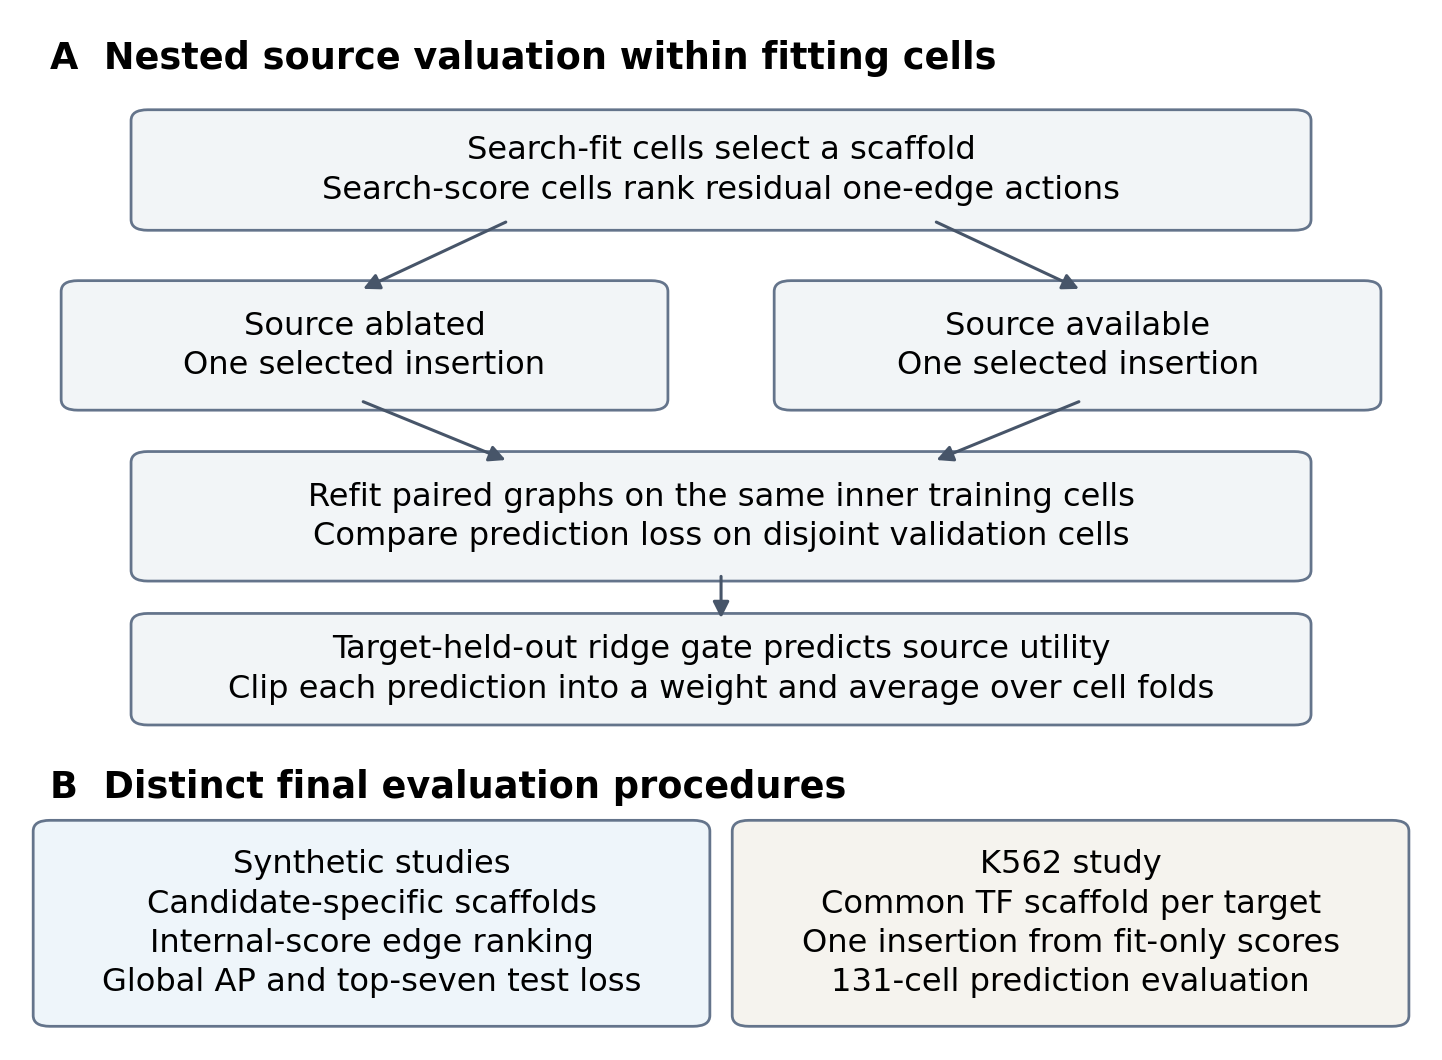
\includegraphics{figures/F01_design.png}
\caption{Figure 1. Source-utility construction and evaluation. The
paired competitors share a scaffold, a candidate universe and one
inserted edge. Source-utility measurement uses validation cells separate
from the action-selection subsets. Target-held-out gate prediction is a
separate grouping layer. The synthetic and K562 studies use different
final selection and evaluation procedures, as detailed in Sections 3.6
and 3.8.}
\end{figure}

\subsection{3.5 Synthetic networks and controlled
evidence}\label{synthetic-networks-and-controlled-evidence}

The first experiment used seeds 2001--2048, balanced over
linear/nonlinear mechanisms, seven genes/140 cells versus nine genes/180
cells, and two source-reliability regimes. Each topologically ordered
graph included predecessor edges independently with probability 0.30,
with random signs and magnitudes uniform on {[}0.35,0.80{]}. Graphs were
redrawn until at least two edges were present, for at most 100 attempts.
Linear expression combined weighted parent values and independent
standard-normal noise. The nonlinear mechanism replaced each parent
contribution with \(1.1w_{ut}\tanh(x_u)\) and, where two parents
existed, added \(0.30\tanh(x_{p_1}x_{p_2})\).

Two simulated sources were explicitly manufactured from the generating
edge truth. Each candidate was observed with probability 0.77. Scores
combined a value of 0.90 or 0.10 according to an effective truth label
with Gaussian noise of standard deviation 0.07, then were clipped to
{[}0,1{]}. In the target-switch regime, alternating target indices
assigned reliability to opposite sources, while the other source
inverted the truth label. In the globally stable regime, sources
independently flipped labels with probabilities 0.12 and 0.25.
Source-generation randomness used seed \(z+888\). Four repeated
conditions retained original evidence, removed 50\% of observed entries,
inverted 25\% of retained scores, or combined both operations.
Corruption used \(v\mapsto1-v\), with source-specific seeds \(z+500\)
and \(z+501\). These were oracle-derived simulations, not independent
biological priors.

The mechanism experiment used 32 new DAGs, seeds 6101--6132, crossed
with saturation absent/present and interaction absent/present. Each DAG
retained identical weights, exogenous noise, source scores and cell
partitions across its four mechanisms. Clean and combined-stress
evidence produced 256 repeated network--condition fits. The explicit
parent-feature experiment repeated that factorial design on seeds
7201--7232.

\subsection{3.6 Synthetic selection, endpoints and
uncertainty}\label{synthetic-selection-endpoints-and-uncertainty}

Synthetic cells were partitioned 60/20/20 by seeded permutation. All
genes were eligible regulators, excluding self-edges. For historical
final edge scoring, each candidate used a two-parent scaffold selected
by absolute training correlation while excluding that candidate
regulator; gains were measured on the internal-score cells. This differs
from the common-scaffold nested source-valuation contexts. Composite
scores ranked all directed candidates globally. Predictive evaluation
refitted models on fit plus internal-score cells using the top seven
ranked edges, then evaluated the reserved test cells. No acyclicity
restriction was imposed on estimated graphs.

Primary edge recovery used noninterpolated average precision (AP)
against the complete simulated reference. The evaluation stage accessed
that reference after rankings were frozen, although simulation truth had
already been used to construct evidence inputs. Secondary endpoints
included AUROC, precision at seven, direction recovery with ties
retained separately and normalized prediction error. Direction accuracy
was the proportion of eligible true-edge pairs for which the true
direction received a strictly higher score than its reverse, among
untied pairs. We report the mean within-network accuracy over assessable
networks and the tie fraction separately; accuracy is undefined if every
pair ties. Pearson, Spearman, conditional-gain and greedy procedures
supplied additional controls. Greedy search used at most 1,600
candidate-loss queries; its reported ranking appended unaccepted
fallback edges, so seven ranked edges need not represent seven accepted
improvements.

Paired effects were summarized per independent DAG. Percentile 95\%
intervals used 4,000 stratified bootstrap resamples, seed 20261125:
eight family-by-size-by-source strata of six DAGs for the first study,
and four size-by-source strata of eight DAGs for each factorial study.
Repeated mechanisms and stresses were not treated as independent
networks. The first primary criterion required a positive lower
AP-difference bound for GCEV minus no\_graph\_state and an upper
relative test-NMSE difference bound of at most 0.02. The mechanism
primary contrast was the interaction effect on that AP difference,
averaged over saturation levels; it additionally required a point effect
of at least 0.02. The parent experiment averaged GCEV minus
no\_parent\_state across four clean mechanisms within each DAG,
requiring an AP effect of at least 0.01, a positive lower bound and the
same 0.02 NMSE bound.

\subsection{3.7 K562 cohort and biological evidence
representations}\label{k562-cohort-and-biological-evidence-representations}

The developmental cohort originated from GEO GSM9224207 and contained
658 source-labelled K562 cells and 60,671 measured genes. The exported
expression matrix was count-like; its exact raw-UMI status remained
unverified. The original split, seed 20261126, retained 394 fitting, 131
internal-score and 133 reserved test cells. After inadequate TF coverage
in an earlier gene universe, a declared developmental redesign selected
16 motif-annotated TFs and 48 additional genes by fitting-cell log1p
variance. Eligibility required at least 5\% detection, positive
variance, an unambiguous primary-chromosome GENCODE v29 protein-coding
annotation {[}23{]} and the locked symbol exclusions. Selection favored
motif-available TFs; the target category excluded motif-eligible
regulators. All 64 genes were prediction targets, giving 1,008 nonself
TF-to-gene candidates.

Motif scores used 17 JASPAR 2026 CORE vertebrate profiles {[}24{]} for
the 16 TFs and 1,201-base GRCh38 promoters, −1000 to +200 relative to
strand-aware gene-level TSSs. Sequences were retrieved from the UCSC
hg38 sequence service {[}25{]}. Both strands were exhaustively scanned
using uniform-background log-odds matrices. The best min--max-scaled
motif score was contrasted with 128 deterministic exact
dinucleotide-preserving promoter shuffles. The prior was the clipped
positive excess above the null median, divided by one minus that median;
a median within \(10^{-10}\) of one yielded zero. The empirical p-value
was the fraction of the 129 observed-plus-null values at least as large
as the observation, with comparison tolerance \(10^{-12}\).
Benjamini-Hochberg adjustment was applied across all 1,008 candidates
{[}26{]}. The continuous scores were not thresholded by adjusted
significance and remained motif potential, not binding labels; all
observed zeros retained observed masks.

DNase context came from two biosamples in ENCODE ENCSR000EOT {[}5{]}.
Each replicate's promoter score was the fraction of promoter bases
covered by the union of its narrowPeak intervals; the source value
averaged both replicates. The primary file pair used different
processing versions. Two matched-version sensitivities and a motif-only
condition were retained. Accessibility was target-specific and broadcast
unchanged across TF candidates. Expression and accessibility originated
from different cultures.

\subsection{3.8 Matched K562 prediction and source-action
audit}\label{matched-k562-prediction-and-source-action-audit}

BIO-V7 used seed 20261127. The primary transformation was \(\log(1+X)\);
a prespecified sensitivity used \(\log(1+10^4X/\text{cell total})\),
with totals over all 60,671 original genes. For every target, two
eligible TFs with highest absolute fitting correlation formed one
scaffold shared by all methods. Residual gains were averaged over three
cell folds while holding this full-fit scaffold fixed. They were
selection statistics, not unbiased validation of scaffold selection.
Seven methods each chose one additional TF per target, yielding 128
scaffold edges and 64 insertions from 880 eligible actions. All eight
transformation-by-prior cases were frozen before internal-score
evaluation.

Ridge coefficients were fitted on the 394 cells. The primary endpoint
averaged normalized squared errors across 64 targets and 131
internal-score cells; the 48 additional targets formed a secondary
endpoint. The primary contrast was GCEV minus no\_graph\_state.
Conditional percentile intervals resampled 131 paired cell-level mean
error differences 10,000 times, seed 20261127. They omitted training
uncertainty and biological-replicate variation; sensitivity contrasts
were descriptive and unadjusted for multiplicity. Reserved test-cell
outcomes and regulatory edge accuracy were not evaluated.

Target-constant additive accessibility cannot change within-target
ordering, since \(S_{ut}+c_t\) and \(S_{ut}\) have the same maximizer.
The implementation explicitly removed such offsets for selection while
preserving original scores. BIO-V8 examined frozen contexts without
fitting or outcome evaluation. Seven representations compared
expression, motif, mean-accessibility-scaled motif, matched
accessibility×motif, permuted accessibility×motif, additive
motif-plus-accessibility and accessibility alone. A single target
permutation used seed 20261128. Product terms were derived interactions,
not additional independent sources. These diagnostics measured whether
representations could alter decisions, not whether altered decisions
improved prediction or regulation.

\section{4 Results}\label{results}

\subsection{4.1 The primary synthetic comparison did not establish a
graph state
advantage}\label{the-primary-synthetic-comparison-did-not-establish-a-graph-state-advantage}

All 48 intended network realizations completed without exclusions.
Across the four source conditions and eleven evaluated methods, the
study produced 2,112 full-universe rankings. The independent
experimental unit was the generated network; repeated source conditions
and method outputs were paired observations within that unit.

On clean source evidence, mean average precision was 0.545860 for GCEV
and 0.538145 for the matched source-feature-only model. Their mean
per-network difference was 0.007715, with a stratified 95\% bootstrap
interval of −0.010750 to 0.026722 (Figure 2). The lower bound did not
exceed zero, so the predeclared AP criterion was not met. GCEV exceeded
the comparator on 21 networks and tied on two. These counts describe the
observed variation and do not replace the primary interval.

The companion mean relative difference in untouched expression-test NMSE
was −0.000804, with an interval of −0.007940 to 0.006036. Its upper
bound satisfied the specified 0.02 noninferiority allowance. Because the
AP criterion failed, the joint primary rule was not satisfied. This
combination illustrates why predictive error and regulatory edge
recovery must be reported separately.

Fixed two-source weighting achieved the highest clean AP among the
eleven evaluated methods in Table 2. GCEV minus fixed weighting was
−0.074505 AP, with a network-bootstrap interval of −0.110828 to
−0.036043. Thus, the added adaptation did not improve clean ranking
recovery in this controlled source setting. Precision at seven was
0.508929 for GCEV, 0.517857 for the no-parent/action-feature model and
0.559524 for fixed two-source weighting. Their mean untied direction
accuracies were 0.578402, 0.579620 and 0.689397, respectively. Pearson
and Spearman tied every eligible reference-pair direction, so their
untied direction accuracy was undefined (Supplementary Table S2).
Pearson correlation had the lowest mean test NMSE (0.844371) and highest
mean AUROC (0.858474) among all eleven methods, despite lower AP than
fixed weighting. These endpoints therefore favored different models.
GCEV exceeded expression-only conditional ranking by 0.048511 AP (95\%
interval 0.023896 to 0.075128) and greedy ranking by 0.049345 AP
(0.012857 to 0.084605). These favorable secondary comparisons do not
isolate the contribution of the explicit parent/action feature block and
do not replace its primary comparison.

\textbf{Table 2. All eleven methods on clean synthetic evidence.} Values
are equal-weight means across 48 generated networks. AP, AUROC and
precision at seven use the complete synthetic edge reference; NMSE uses
untouched expression-test cells. Higher ranking metrics and lower NMSE
are preferable. Legacy single-source controls use only the primary
prior.

\begin{longtable}[]{@{}
  >{\raggedright\arraybackslash}p{(\columnwidth - 8\tabcolsep) * \real{0.2000}}
  >{\raggedleft\arraybackslash}p{(\columnwidth - 8\tabcolsep) * \real{0.2000}}
  >{\raggedleft\arraybackslash}p{(\columnwidth - 8\tabcolsep) * \real{0.2000}}
  >{\raggedleft\arraybackslash}p{(\columnwidth - 8\tabcolsep) * \real{0.2000}}
  >{\raggedleft\arraybackslash}p{(\columnwidth - 8\tabcolsep) * \real{0.2000}}@{}}
\toprule\noalign{}
\begin{minipage}[b]{\linewidth}\raggedright
Method
\end{minipage} & \begin{minipage}[b]{\linewidth}\raggedleft
AP
\end{minipage} & \begin{minipage}[b]{\linewidth}\raggedleft
AUROC
\end{minipage} & \begin{minipage}[b]{\linewidth}\raggedleft
Precision at 7
\end{minipage} & \begin{minipage}[b]{\linewidth}\raggedleft
Test NMSE
\end{minipage} \\
\midrule\noalign{}
\endhead
\bottomrule\noalign{}
\endlastfoot
Fixed two-source weighting & 0.620365 & 0.828134 & 0.559524 &
0.878056 \\
Legacy single-source fixed & 0.596476 & 0.818221 & 0.532738 &
0.875504 \\
Full GCEV & 0.545860 & 0.802644 & 0.508929 & 0.859175 \\
Legacy single-source heuristic & 0.533077 & 0.798141 & 0.497024 &
0.855846 \\
Global source weighting & 0.523710 & 0.800305 & 0.514881 & 0.861103 \\
Legacy single-source adaptive & 0.520019 & 0.819785 & 0.502976 &
0.849593 \\
No parent or action features & 0.538145 & 0.806540 & 0.517857 &
0.860085 \\
Expression-only conditional & 0.497349 & 0.793515 & 0.482143 &
0.855729 \\
Greedy expression model & 0.496515 & 0.795693 & 0.461310 & 0.851707 \\
Absolute Pearson correlation & 0.453455 & 0.858474 & 0.538690 &
0.844371 \\
Absolute Spearman correlation & 0.446882 & 0.852002 & 0.532738 &
0.847077 \\
\end{longtable}

\begin{figure}
\centering
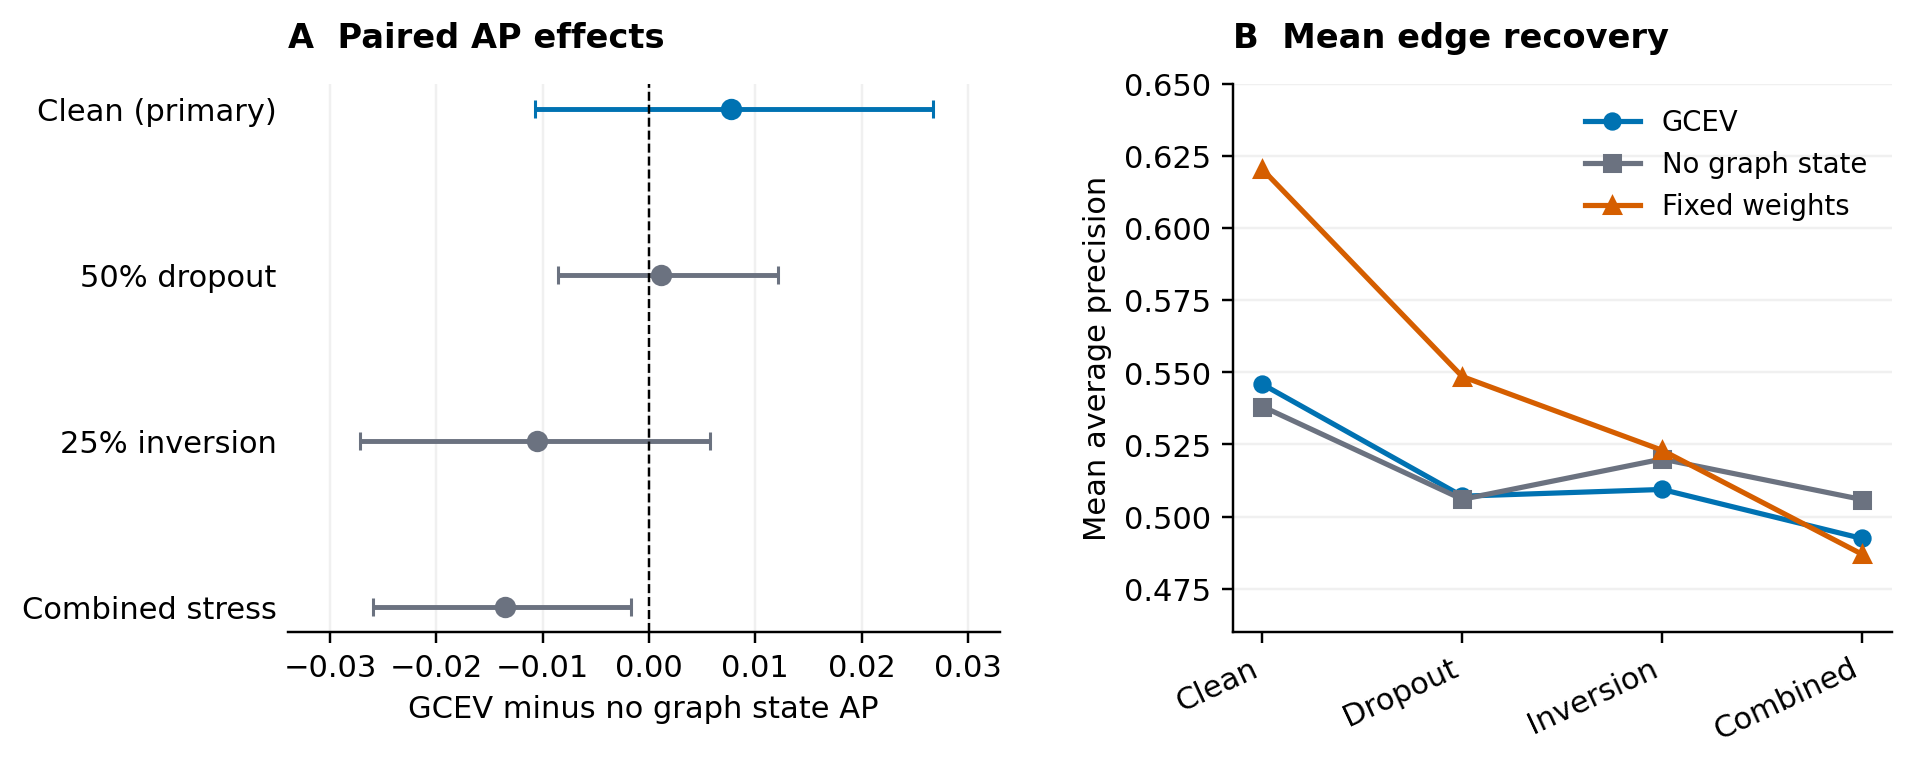
\includegraphics{figures/F02_synthetic_evaluation.png}
\caption{Figure 2. Synthetic edge-ranking comparisons across the four
predeclared source conditions. Panel A shows mean paired
GCEV-minus-no-graph-state AP differences with network-stratified 95\%
bootstrap intervals. The clean comparison is primary; stress comparisons
are secondary. Panel B shows mean AP for GCEV, the no-graph-state model
and fixed weighting. The four conditions reuse the same 48 networks.}
\end{figure}

\subsection{4.2 Source stress altered performance without establishing a
robustness
advantage}\label{source-stress-altered-performance-without-establishing-a-robustness-advantage}

With 50\% source dropout, the GCEV-minus-no-graph-state difference was
0.001087 AP, with an interval of −0.008541 to 0.012163. With 25\% score
inversion, the difference was −0.010545, with an interval of −0.027204
to 0.005771. Under combined dropout and inversion, it was −0.013503,
with an interval of −0.025987 to −0.001651. The combined-condition
interval excluded zero in the unfavorable direction, but this was a
secondary contrast without a separate multiplicity-adjusted confirmatory
claim.

Fixed weighting decreased from 0.620365 AP in the clean condition to
0.486952 under combined stress. GCEV decreased from 0.545860 to
0.492404. The smaller decline for GCEV does not establish a better
endpoint under stress: its combined-condition difference from fixed
weighting was only 0.005452 AP, with an interval of −0.021591 to
0.033662. We therefore interpret the results as different sensitivity
patterns rather than demonstrated robustness superiority.

Exploratory stratification suggested a clean GCEV-minus-no-graph-state
effect of −0.0253 AP in linear networks and 0.0407 in nonlinear
networks. These observations motivated a subsequent mechanism test. They
were not predeclared subgroup superiority results and were not
substituted for the unsuccessful primary comparison.

\subsection{4.3 Neither follow up study met its primary
criterion}\label{neither-follow-up-study-met-its-primary-criterion}

The mechanism experiment used 32 new network seeds and paired linear,
saturation, interaction and combined mechanisms. Its primary estimand
was a difference in the incremental graph-state effect between
interaction-present and interaction-absent mechanisms. The observed
interaction effect was −0.002080 AP, with a 95\% interval of −0.016369
to 0.011090. It failed both the positive-lower-bound criterion and the
minimum 0.020 AP point-effect threshold. Consequently, this experiment
did not confirm that two-parent interactions explained the earlier
favorable nonlinear subgroup.

In the interaction-containing mechanism settings, the mean relative
test-NMSE contrast was −0.006976 (95\% interval −0.012342 to −0.001930),
satisfying the 0.02 noninferiority allowance. This favorable predictive
contrast concerns a different endpoint from the unsuccessful interaction
AP criterion.

The separate 32-network explicit parent-feature ablation compared full
GCEV with a model retaining source and action features but omitting
parent count and parent-target correlation. Averaging across the four
clean mechanisms within each network gave an AP difference of 0.005644,
with an interval of −0.000168 to 0.011448. The positive-lower-bound and
minimum 0.010 AP requirements were not met (Table 3). Its relative
test-NMSE contrast was 0.000700 (95\% interval −0.002264 to 0.003817),
also satisfying the noninferiority allowance. Neither later study met
its joint primary success rule.

\textbf{Table 3. Primary results of the three synthetic studies.} Each
interval resamples independently generated networks within the declared
strata. The estimands differ and are not pooled. Relative NMSE contrasts
use the corresponding locked aggregation rules.

\begin{longtable}[]{@{}
  >{\raggedright\arraybackslash}p{(\columnwidth - 8\tabcolsep) * \real{0.2000}}
  >{\raggedright\arraybackslash}p{(\columnwidth - 8\tabcolsep) * \real{0.2000}}
  >{\raggedleft\arraybackslash}p{(\columnwidth - 8\tabcolsep) * \real{0.2000}}
  >{\raggedright\arraybackslash}p{(\columnwidth - 8\tabcolsep) * \real{0.2000}}
  >{\raggedright\arraybackslash}p{(\columnwidth - 8\tabcolsep) * \real{0.2000}}@{}}
\toprule\noalign{}
\begin{minipage}[b]{\linewidth}\raggedright
Study and network count
\end{minipage} & \begin{minipage}[b]{\linewidth}\raggedright
Primary AP estimand
\end{minipage} & \begin{minipage}[b]{\linewidth}\raggedleft
Estimate
\end{minipage} & \begin{minipage}[b]{\linewidth}\raggedright
95\% interval
\end{minipage} & \begin{minipage}[b]{\linewidth}\raggedright
Primary rule
\end{minipage} \\
\midrule\noalign{}
\endhead
\bottomrule\noalign{}
\endlastfoot
Main comparison, 48 & GCEV minus no graph state, clean & 0.007715 &
−0.010750 to 0.026722 & Not met \\
Mechanism, 32 & Interaction difference in graph-state benefit &
−0.002080 & −0.016369 to 0.011090 & Not met \\
Parent ablation, 32 & GCEV minus no parent state, clean & 0.005644 &
−0.000168 to 0.011448 & Not met \\
\end{longtable}

The parent-feature diagnosis limits the breadth of this negative
finding. Parent count equalled two in all 256 condition-specific
datasets, and therefore could not explain variation in source utility.
Parent-target correlation varied, with mean within-condition standard
deviation 0.1088, but adding the block did not produce the required
advantage. Action features still depended on a scaffold. Removing the
explicit parent block therefore did not remove every pathway through
which graph information entered the learner.

\subsection{4.4 K562 priors had distinct coverage and interpretation
limits}\label{k562-priors-had-distinct-coverage-and-interpretation-limits}

All 64 promoter windows and 17 selected motifs were available for the
1,008 nonself TF-to-gene candidates. The motif procedure assigned
positive continuous scores to 517 candidates. Forty-seven candidates had
nominal empirical p-values below 0.05, but none passed a
Benjamini-Hochberg threshold of q below 0.05; the smallest adjusted
value was 0.853984. The continuous scores were retained as
sequence-derived binding-potential features rather than thresholded
discoveries or binding probabilities.

The original DNase files overlapped 47 promoters in one replicate and 41
in the other; 41 promoters overlapped both, and 17 overlapped neither.
Mean accessibility across the 64 promoters was 0.171101. The original
files used different peak-calling versions. Matched-version
sensitivities retained 41 promoters with overlaps in both replicates but
changed mean accessibility to 0.190095 and 0.146844. These are
processing sensitivities within one DNase experiment, rather than
independent biological replications.

\subsection{4.5 The real expression comparison did not establish
incremental predictive
benefit}\label{the-real-expression-comparison-did-not-establish-incremental-predictive-benefit}

Seven methods were evaluated under eight prespecified
transformation-by-prior conditions. Within each condition, every method
used the same 128 scaffold edges and selected 64 insertions, yielding
192-edge predictive graphs. All 3,584 target-level choices were frozen
before the 131-cell readout. Reserved test cells were not used for
fitting, selection or performance evaluation.

For the primary original-expression scale and original DNase processing
combination, GCEV NMSE was 0.402598, compared with 0.402822 for the
no-graph-state model (Table 4). The paired difference was −0.000223,
with a conditional 95\% cell-bootstrap interval of −0.000636 to
0.000175. GCEV-minus-fixed and GCEV-minus-expression-only differences
were 0.000473 and 0.001023, respectively, with intervals spanning zero
(Figure 3). These estimates provide no clear primary-case advantage for
full GCEV.

\textbf{Table 4. K562 primary-case prediction and graph choices.} NMSE
averages errors on 131 internal-score cells, normalized by fitting-cell
target variance. The additional-target column excludes the 16 candidate
TFs from the error average. Insertions are compared with expression-only
selection; all graphs retain the same scaffold.

\begin{longtable}[]{@{}
  >{\raggedright\arraybackslash}p{(\columnwidth - 6\tabcolsep) * \real{0.2500}}
  >{\raggedleft\arraybackslash}p{(\columnwidth - 6\tabcolsep) * \real{0.2500}}
  >{\raggedleft\arraybackslash}p{(\columnwidth - 6\tabcolsep) * \real{0.2500}}
  >{\raggedleft\arraybackslash}p{(\columnwidth - 6\tabcolsep) * \real{0.2500}}@{}}
\toprule\noalign{}
\begin{minipage}[b]{\linewidth}\raggedright
Method
\end{minipage} & \begin{minipage}[b]{\linewidth}\raggedleft
NMSE across 64 genes
\end{minipage} & \begin{minipage}[b]{\linewidth}\raggedleft
NMSE across 48 additional targets
\end{minipage} & \begin{minipage}[b]{\linewidth}\raggedleft
Changed insertions
\end{minipage} \\
\midrule\noalign{}
\endhead
\bottomrule\noalign{}
\endlastfoot
Expression only & 0.401575 & 0.368196 & 0 \\
Fixed sources & 0.402125 & 0.366089 & 33 \\
Global source gate & 0.401575 & 0.368196 & 0 \\
No graph state & 0.402822 & 0.368196 & 2 \\
No parent state & 0.402598 & 0.367898 & 3 \\
No action state & 0.401324 & 0.368196 & 2 \\
Full GCEV & 0.402598 & 0.367898 & 3 \\
\end{longtable}

The no-action-state model had the lowest primary point error, but it was
not promoted to the primary method after evaluation. Full GCEV and the
no-parent-state model selected identical primary graphs. The target-only
error summary also differed from the all-gene summary: fixed weighting
had the lowest point NMSE among the seven models on the 48 additional
targets. These changes reinforce the importance of retaining the
predeclared endpoint and reporting its sensitivities.

\begin{figure}
\centering
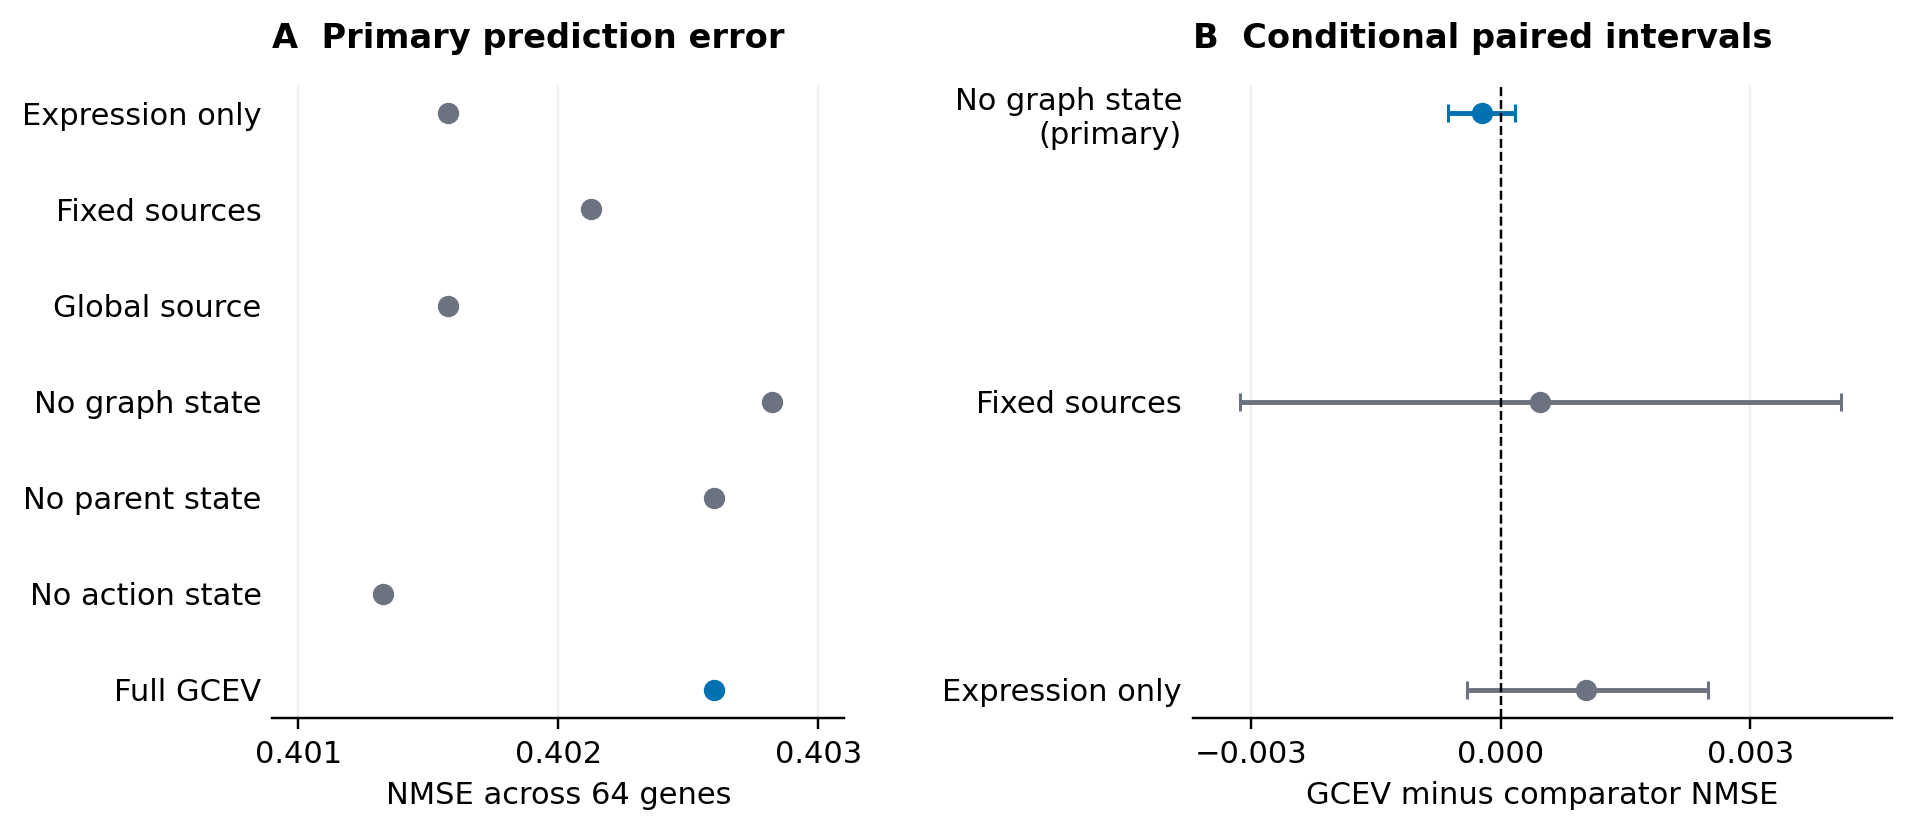
\includegraphics{figures/F03_k562_prediction.png}
\caption{Figure 3. Developmental K562 prediction. Panel A displays
primary-case NMSE for all seven methods. Panel B shows
GCEV-minus-comparator differences and conditional paired-cell 95\%
bootstrap intervals. Negative differences favor GCEV. The intervals
condition on the selected genes, fitted models and one cohort; they do
not quantify between-culture variation or model-training uncertainty.}
\end{figure}

The two matched DNase versions preserved full GCEV's primary-scale
choices. Removing DNase entirely altered the learned contexts:
motif-only GCEV NMSE was 0.403298 versus 0.401852 for the no-graph-state
model, a difference of 0.001446 with interval −0.000177 to 0.003121.
This does not isolate an independently confirmed accessibility
mechanism.

On the full-library normalized sensitivity scale, GCEV NMSE was
0.699570, the no-graph-state value was 0.699506 and the fixed-source
value was 0.706015. GCEV-minus-fixed was −0.006444, with interval
−0.011730 to −0.001303. In contrast, GCEV-minus-no-graph-state was
0.000065, with interval −0.000575 to 0.000726. The favorable
fixed-comparator sensitivity did not replace the primary graph-state
comparison. Absolute NMSE values across transformations concern
different transformed responses and variance denominators and should not
be read as a direct competition between preprocessing schemes.

\subsection{4.6 Evidence influence and learned weight were not
equivalent to
utility}\label{evidence-influence-and-learned-weight-were-not-equivalent-to-utility}

Accessibility was constant across candidate TFs for each target. Its
additive contribution therefore cancelled from every within-target score
difference. In each two-source K562 condition, adding accessibility
changed zero of the 192 nested source-present versus source-ablated
choices, and all observed accessibility utility labels were zero.
Nevertheless, the shared ridge gate predicted positive accessibility
weights for 47 of 64 primary targets, with mean weight 0.035305. Such
predictions can arise from the shared regression fitted across
source-target rows. They are not observations of accessibility utility.

Motif inclusion changed 96 of 192 nested choices on the original scale.
Its mean paired utility was −0.003427, while the mean learned motif
weight was 0.039244 and 39 targets received positive weights. Thus, the
ability of a source to change a choice did not establish that its
changed choices improved prediction on average. The clipping and
averaging used to construct the weights also prevent their
interpretation as calibrated utility estimates or probabilities.

The saved-output diagnosis compared seven representations at fixed
coefficient 0.3. In the primary case, motif alone changed 33 of 64
decisions relative to expression-only scoring. Multiplying motif scores
by global mean accessibility changed nine; multiplying by matched target
accessibility changed eight; and multiplying by a frozen permutation of
accessibility also changed eight (Figure 4). Equal counts did not imply
identical choices: the matched and permuted representations differed
from each other at eight targets. Their predictive errors and biological
accuracy were not evaluated.

\textbf{Table 5. Primary representation diagnosis.} Counts refer to 64
target-specific selections from already saved residual candidates. They
quantify action influence at fixed coefficient 0.3, not learned-model
performance or a new expression evaluation.

\begin{longtable}[]{@{}
  >{\raggedright\arraybackslash}p{(\columnwidth - 4\tabcolsep) * \real{0.3333}}
  >{\raggedleft\arraybackslash}p{(\columnwidth - 4\tabcolsep) * \real{0.3333}}
  >{\raggedleft\arraybackslash}p{(\columnwidth - 4\tabcolsep) * \real{0.3333}}@{}}
\toprule\noalign{}
\begin{minipage}[b]{\linewidth}\raggedright
Representation
\end{minipage} & \begin{minipage}[b]{\linewidth}\raggedleft
Targets with TF-varying source scores
\end{minipage} & \begin{minipage}[b]{\linewidth}\raggedleft
Choices changed from expression only
\end{minipage} \\
\midrule\noalign{}
\endhead
\bottomrule\noalign{}
\endlastfoot
Accessibility only & 0 & 0 \\
Motif only & 64 & 33 \\
Motif plus accessibility & 64 & 33 \\
Global mean accessibility times motif & 64 & 9 \\
Matched target accessibility times motif & 47 & 8 \\
Permuted target accessibility times motif & 47 & 8 \\
\end{longtable}

\begin{figure}
\centering
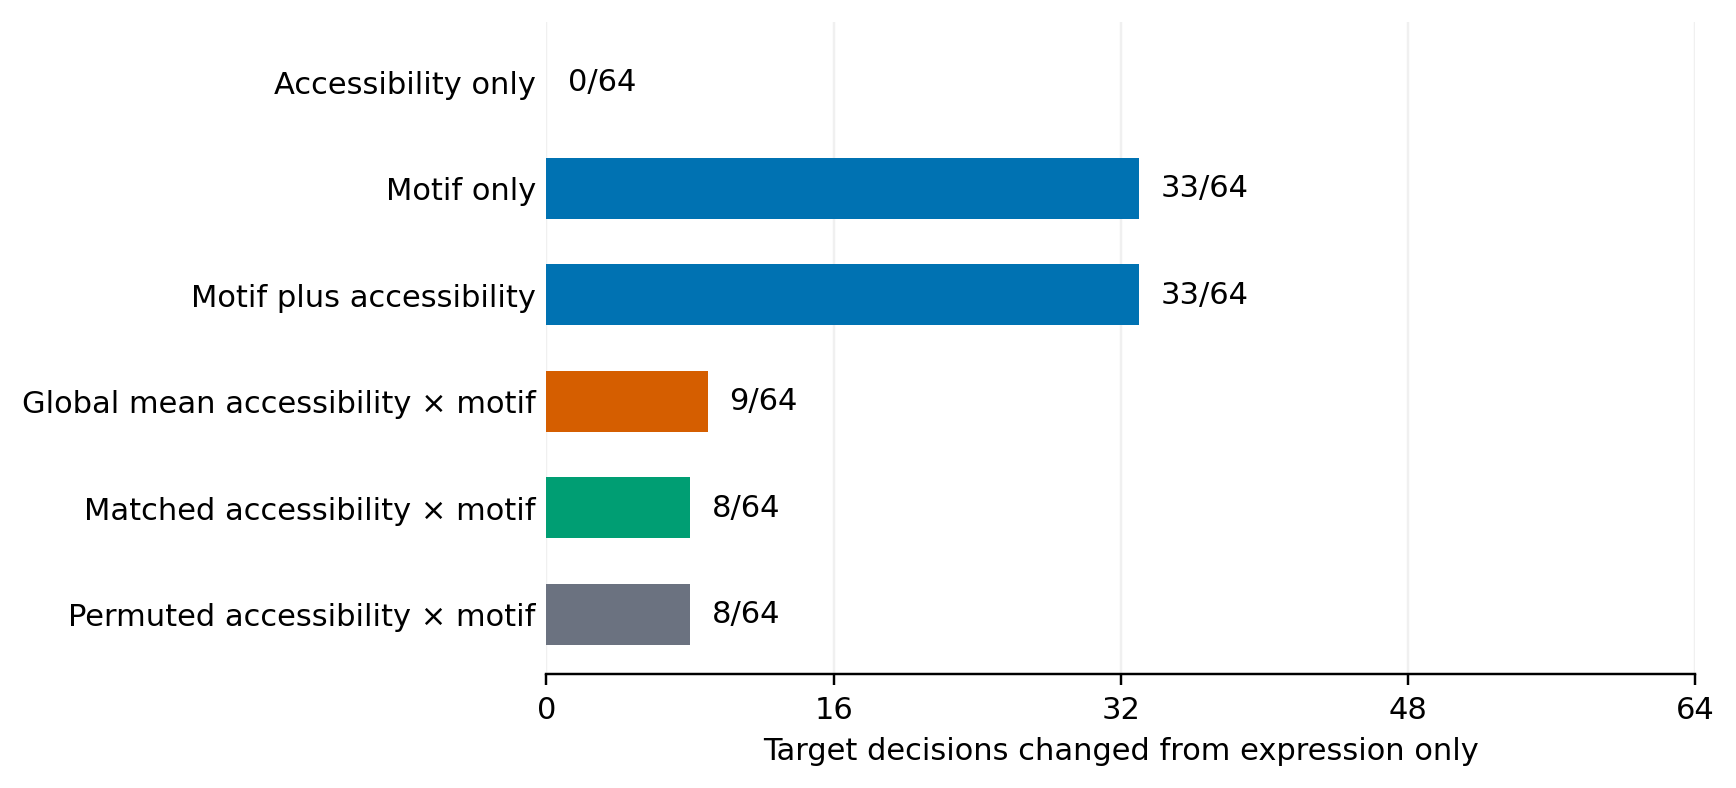
\includegraphics{figures/F04_source_influence.png}
\caption{Figure 4. Action influence of alternative evidence
representations. Bars show the number of primary-case target decisions
changed relative to expression-only selection, out of 64.
Target-constant additive accessibility changes no decisions.
Multiplicative accessibility rescales motif relative to expression and
can change their combined choice; these counts do not measure
usefulness. The matched and permuted representations are fixed
saved-score diagnostics.}
\end{figure}

The invariance held across both expression transformations and all three
accessibility versions: accessibility-only scoring preserved
expression-only choices in all 384 target cases, and additive
motif-plus-accessibility scoring preserved motif-only choices in all
384. Positive multiplicative accessibility preserved motif ordering
within a target while changing motif's scale relative to expression. A
zero accessibility value removed that motif contribution. The product
remained a derived representation of two sources, not a third
independent assay.

\subsection{4.7 Reproduction supported numerical correctness within the
executed
settings}\label{reproduction-supported-numerical-correctness-within-the-executed-settings}

The synthetic execution audit recomputed ranking metrics for all 2,112
outputs of the 48-network study, with maximum discrepancy 1.11 × 10⁻¹⁶.
Independent-environment K562 reproduction recovered all 3,584 choices,
56 method summaries and 24 contrasts, with zero reported differences in
summaries and contrasts. A separate primary-case linear-algebra audit
reproduced 448 regressions with maximum individual normalized-error
discrepancy 2.98 × 10⁻¹⁴.

The saved-output diagnosis preserved 49,280 legacy residual-score rows
and checked 2,688 representation-specific decisions. These checks
support numerical reproduction and alignment of the comparisons. They
neither add independent experimental units nor establish that the
predictions correspond to biological regulation.

GCEV incurred additional fitting work. The 48-network study recorded 189
nested source-valuation loss evaluations for seven-gene networks and 297
for nine-gene networks. Fixed weighting does not perform an equivalent
utility-learning stage. Matching candidate sets and inserted-edge
budgets therefore did not match total training computation. No claim of
computational-efficiency superiority follows from the reported
performance comparisons.

\section{5 Discussion}\label{discussion}

\subsection{5.1 What the controlled comparisons
establish}\label{what-the-controlled-comparisons-establish}

The three synthetic studies did not establish the proposed primary
advantage of the tested graph-state representation. The real-expression
comparison likewise did not show a clear incremental prediction benefit
under its primary analysis. Together, these results constrain a specific
formulation: a ridge model predicting paired one-edit source utility
from the selected source, parent and action features, followed by
clipped weighting. They do not establish equivalence to the controls or
exclude useful effects under other representations and data regimes.

The fixed-weight result deserves particular attention. The synthetic
priors were deliberately informative and derived from complete simulated
truth. A fixed contribution could exploit this information without
estimating a utility model from a small number of source-target
observations. GCEV's utility labels instead rewarded expression
prediction after an edit. These objectives need not align: a source that
helps rank a true edge can have limited incremental predictive benefit
when correlated parents already explain the target. The opposing
ordering of methods by AP and NMSE is consistent with this distinction,
although the experiments do not identify it as the sole cause of
underperformance.

The subsequent mechanism study improved the interpretation of an
initially favorable subgroup. The nonlinear-versus-linear difference in
the first study could have encouraged a broader claim about
interaction-aware inference. Testing a specified interaction estimand on
new seeds did not support that explanation. Reporting the failed
follow-up preserves the difference between a pattern that generates a
hypothesis and evidence that confirms it.

\subsection{5.2 A source must be able to affect the decision being
valued}\label{a-source-must-be-able-to-affect-the-decision-being-valued}

The accessibility diagnosis clarifies three separate questions. Is
evidence observed? Can it change the decision? Do the resulting changes
improve an evaluation outcome? Accessibility was observed for the chosen
promoters, but its additive target-constant representation could not
alter a within-target TF ranking. Motif scores could alter that ranking,
but their mean nested utility was negative. Neither availability nor
influence established usefulness.

The cancellation result follows directly from the scoring equation and
is not a new mathematical theorem. Its value here is empirical and
methodological: it identifies why a source-use interpretation would be
invalid for this executed decision rule. Positive accessibility weights
could otherwise be mistaken for learned support for that modality. The
shared gate's predictions describe its regression behavior, rather than
measured causal effects or calibrated source reliability.

Recent multimodal benchmarking has similarly emphasized testing the
contribution of each modality {[}15{]}. Our local analysis complements
such evaluations by specifying the decision set on which invariance
holds. A target-dependent offset may matter when edges to different
targets compete in a global ranking, even though it cancels when
candidate TFs compete for one fixed target. The BIO-V8 analysis
therefore retained the original across-target ranking score separately
from the within-target action score. It did not overwrite a legacy
ranking using an equivalence that holds only for a different decision
problem.

An interaction between accessibility and motif can avoid the additive
invariance, but introduces another question. Positive target
accessibility scales all motif scores at that target equally. A
reduction in changed choices may therefore result simply from
attenuation relative to the expression score. Comparing matched
accessibility with both a global-mean attenuation and a fixed
permutation helps identify this ambiguity. In the present diagnosis,
matched and permuted counts alone provide no evidence of a biological
matching benefit. Evaluating that benefit would require newly locked
predictive or biological endpoints.

\subsection{5.3 Limits of graph state and source utility
estimation}\label{limits-of-graph-state-and-source-utility-estimation}

The explicit parent feature set was small, and its parent-count
component was constant by design. The action features retained indirect
information about the scaffold, so the parent ablation estimated the
value of two explicit columns rather than the value of graph information
in general. The experiments do not test variable-size parent sets,
learned graph embeddings, global topology or a sequential policy.
Conclusions about those alternatives would require different
experiments.

The utility learner also faces sparse and heterogeneous labels. A label
is exactly zero whenever the source-present and source-ablated
procedures select the same action. When they select different actions,
the difference is measured on a relatively small validation fold and
clipped to a bounded range. The model pools rows across sources and
predicts for held-out targets; source indicators and features do not
guarantee exact zero predictions for a source with zero observed
utility. The subsequent weight map removes negative predictions and
saturates sufficiently positive values. These properties can generate
weights whose interpretation differs from either mean observed utility
or an edge's probability of being correct.

Target-held-out learning prevents a target's own utility labels from
fitting its predictor, but does not make genes biologically independent.
Genes share cells, sources and scaffold construction. Likewise, nested
contexts differ from the final graph contexts to which the averaged
weights are applied. These are potential sources of error and limits on
interpretation; their individual causal contributions were not isolated
by the completed experiments.

\subsection{5.4 Scope of the biological
evidence}\label{scope-of-the-biological-evidence}

The real-data analysis uses a single source-labelled K562 cohort,
selected genes and a constrained one-insertion graph. Its uncertainty
intervals condition on the fitted models and observed cells. They do not
account for training variability, gene-selection uncertainty or
variation across independently collected cultures. The reserved 133 test
cells were not analyzed in this manuscript. Their future use could
provide a final within-cohort predictive readout, but would still not
establish transfer to another biological setting.

The priors have additional limits. Gene-level promoter coordinates are
not verified active-transcript starts in these cells. A positive motif
score is not evidence of occupied binding, and no edge passed the stated
motif multiple-testing threshold. DNase coverage describes promoter
accessibility rather than TF-specific occupancy; expression and
accessibility came from different K562 cultures. Full publication-level
assay QC and the lineage of potentially overlapping prior and reference
experiments remain incomplete.

No qualified independent binding or perturbation panel was used to score
the inferred real edges. Accordingly, we report no real-data AP, AUROC,
F1 or causal-recovery metric. Previously inspected perturbation results
cannot retrospectively become untouched confirmation. Binding,
perturbation response and expression prediction would also require
separate interpretations if future evaluation data become available. The
operational difficulty of retrieving external assay metadata is an
acquisition limitation, not evidence that an assay or regulatory
relation is absent.

\subsection{5.5 Implications for further
evaluation}\label{implications-for-further-evaluation}

The next computational evaluation should address the limitations that
matter for the claim: larger and materially different network-generating
systems, meaningful variation in parent state, and relevant external
inference baselines. The current simulations isolate selected components
but do not constitute broad biological benchmarking. Repeating more
seeds within the same seven- and nine-gene framework would improve Monte
Carlo precision without addressing that limitation.

If the objective is to improve the source-valuation method, two
hypotheses are suggested by the completed analyses: learning source
utility with a representation aligned to the actual decision set, and
modeling zero-utility or source-specific behavior more explicitly. These
are hypotheses for future study, not validated fixes. Their assessment
should use new locked outcomes rather than repeatedly tune on the
present synthetic seeds or K562 evaluation partition.

\section{6 Conclusion}\label{conclusion}

We evaluated whether selected graph-state features improve adaptive
weighting of biological evidence in a one-step GRN inference procedure.
Three prospectively locked synthetic studies did not meet their primary
success criteria, and the developmental K562 comparison did not
establish an incremental predictive advantage. Fixed source weighting
was stronger on clean synthetic edge recovery. A saved-output diagnosis
showed that target-constant additive accessibility could not influence
the within-target action being valued, although the learned gate
assigned it positive weights. Alternative multiplicative representations
changed decisions without establishing that those changes were useful.
The findings support a scoped account of the tested formulation and
motivate evaluating evidence availability, action influence and
predictive or biological utility as separate quantities.

\section{Data and code availability}\label{data-and-code-availability}

The public research repository is
https://github.com/TshepoGobonamang/bio-rl-grn {[}27{]}. The evidence
snapshot used for this manuscript is commit
\texttt{4328d45ec196a1dc05d46a6e36dc8480810597cb}. Stage-specific
implementation commits, prospectively locked configurations, source
identifiers and reproduction instructions are listed in Supplementary
Table S1 and the accompanying evidence ledger. Earlier synthetic
experiments require their recorded implementation versions because
subsequent development expanded the method grid and adapted the
real-data scaffold. Public biological sources comprise GEO GSM9224207
within GSE306708, GENCODE v29, UCSC hg38 sequence, the selected JASPAR
2026 motifs and ENCODE experiment ENCSR000EOT. The source manifests
retain exact file identifiers and checksums. No new expression or
perturbation experiment was conducted for the manuscript preparation.

\section{Supplementary information}\label{supplementary-information}

\subsection{S1 Protocol freezes and computational
reproduction}\label{s1-protocol-freezes-and-computational-reproduction}

\textbf{Supplementary Table S1. Protocol and implementation versions.}

Commit links identify exact immutable repository versions. ``Locked''
denotes a repository precommit, not registration with an independent
registry. Auditing saved rankings and rerunning the same source bytes
establish computational reproduction, not biological replication.

\begin{longtable}[]{@{}
  >{\raggedright\arraybackslash}p{(\columnwidth - 6\tabcolsep) * \real{0.2500}}
  >{\raggedright\arraybackslash}p{(\columnwidth - 6\tabcolsep) * \real{0.2500}}
  >{\raggedright\arraybackslash}p{(\columnwidth - 6\tabcolsep) * \real{0.2500}}
  >{\raggedright\arraybackslash}p{(\columnwidth - 6\tabcolsep) * \real{0.2500}}@{}}
\toprule\noalign{}
\begin{minipage}[b]{\linewidth}\raggedright
Experiment
\end{minipage} & \begin{minipage}[b]{\linewidth}\raggedright
Protocol record
\end{minipage} & \begin{minipage}[b]{\linewidth}\raggedright
Implementation or prediction freeze
\end{minipage} & \begin{minipage}[b]{\linewidth}\raggedright
Reproduction evidence
\end{minipage} \\
\midrule\noalign{}
\endhead
\bottomrule\noalign{}
\endlastfoot
48-DAG comparison; seeds 2001--2048 & Narrative/JSON:
\href{https://github.com/TshepoGobonamang/bio-rl-grn/commit/cb7b3d2aff6827c98c370ba14fbc19293405a1c3}{cb7b3d2}
& Code/tests/workflow:
\href{https://github.com/TshepoGobonamang/bio-rl-grn/commit/c4d98e9b48c5fd99dc0d630d39003ac2d2f559e8}{c4d98e9}
& Independent rescore of 2,112 rankings; zero failures; maximum AP/AUROC
discrepancy \(1.11\times10^{-16}\). \\
32-DAG mechanism factorial; seeds 6101--6132 & Narrative:
\href{https://github.com/TshepoGobonamang/bio-rl-grn/commit/f446a3d8764148dbfc4a885f334004bb74318fba}{f446a3d};
executable JSON:
\href{https://github.com/TshepoGobonamang/bio-rl-grn/commit/0178b372b7b532f25b0aa187a360e256774c95ca}{0178b37}
& Runner:
\href{https://github.com/TshepoGobonamang/bio-rl-grn/commit/eeb7c126638cef61af8ec3baa39bb523c1873e8c}{eeb7c12};
complete pre-evaluation code/configuration/workflow checkout:
\href{https://github.com/TshepoGobonamang/bio-rl-grn/commit/7857ad6b020621cfdf45ca744ddc852df04a8a32}{7857ad6}
& Independent local audit of 2,816 rankings; all AP/AUROC reconciled
within \(10^{-11}\); no DAG failure. \\
32-DAG parent-feature ablation; seeds 7201--7232 & Narrative:
\href{https://github.com/TshepoGobonamang/bio-rl-grn/commit/b77f235a2efd0d10a100413c5bf8ddc59a72cdd1}{b77f235}
& Executable JSON/code:
\href{https://github.com/TshepoGobonamang/bio-rl-grn/commit/bf185df34efbd0262c0ff3c2c779dde2265234ca}{bf185df}
& Completed local evaluation and independent rescore of 3,328 rankings.
The cited record does not establish the separate GitHub full-run
outcome. \\
K562 matched prediction, BIO-V7 & Protocol:
\href{https://github.com/TshepoGobonamang/bio-rl-grn/commit/41baca2de083b8b13ed602bcfcbf804e910f71cb}{41baca2}
& Implementation:
\href{https://github.com/TshepoGobonamang/bio-rl-grn/commit/d136b66dfb59a6cde055f40668d56202a8806b7a}{d136b66};
all prediction choices:
\href{https://github.com/TshepoGobonamang/bio-rl-grn/commit/ac5c86c820ec2b2178f769639d1e5c0e7de24ade}{ac5c86c}
& Run
\href{https://github.com/TshepoGobonamang/bio-rl-grn/actions/runs/46004482269}{46004482269}
at
\href{https://github.com/TshepoGobonamang/bio-rl-grn/commit/77d0552c2a885540e5e665d541dbd4d7f7eafd91}{77d0552}:
identical 3,584 choices; zero differences in 56 summaries and 24
contrasts. \\
Saved-score evidence qualification, BIO-V8 & Follow-up design:
\href{https://github.com/TshepoGobonamang/bio-rl-grn/commit/9169be40c3658d45178ed170587f5058ad8c9942}{9169be4}
& Implementation:
\href{https://github.com/TshepoGobonamang/bio-rl-grn/commit/eb3ca377bbbf02e7577c3f0aab6eca31cd61085f}{eb3ca37}
& Run
\href{https://github.com/TshepoGobonamang/bio-rl-grn/actions/runs/46011226484}{46011226484}
at the implementation commit: eight output tables byte-identical. No new
prediction or biological outcome evaluation. \\
\end{longtable}

Later code expanded the synthetic comparator grid; reproducing the
historical 11-method outputs therefore requires the corresponding
historical version. BIO-V7 introduced a separately declared
TF-constrained adaptation. BIO-V8 followed known developmental outcomes
and cannot be interpreted as an independent retrospective confirmation.
Its external metadata inventory remained incomplete after six HTTP 403
responses. Workflow artifacts have finite retention; they are not a
permanent archival release.

\subsection{S2 Exact estimands and implementation
details}\label{s2-exact-estimands-and-implementation-details}

For network \(j\), let \(E_{Gj}\) and \(E_{Bj}\) be test NMSE for GCEV
and its specified comparator. Relative prediction error is

\[
\rho_j=(E_{Gj}-E_{Bj})/\max(E_{Bj},\epsilon),
\]

with \(\epsilon=10^{-12}\) in the 48-network script and \(10^{-10}\) in
the factorial scripts. The statistic averages these paired relative
differences; it is not the relative difference of grand means.

For saturation \(a\in\{0,1\}\), interaction \(b\in\{0,1\}\), and
\(d_{jab}=AP_{G,jab}-AP_{\mathrm{no\_graph\_state},jab}\), the clean
mechanism estimand is

\[
\theta_{\mathrm{mean}}=\frac1{32}\sum_j\frac12
\left((d_{j01}-d_{j00})+(d_{j11}-d_{j10})\right).
\]

Its accompanying NMSE contrast averages \((\rho_{j01}+\rho_{j11})/2\)
within each DAG. The parent study instead averages GCEV-minus-no-parent
AP and relative NMSE across all four clean mechanisms within each DAG,
then across the 32 DAGs. Bootstrap resampling preserves these DAG-level
paired units.

The motif null seed is the big-endian integer represented by the first
eight SHA256 bytes of the UTF-8 string formed by the protocol
identifier, a pipe separator and the \textbf{target gene symbol}, not
its Ensembl ID. Canonical A/C/G/T iteration fixes shuffle
reproducibility. With 128 null scores,

\[
p=\frac{1+\#\{v_{\mathrm{null}}\ge v_{\mathrm{observed}}-10^{-12}\}}{129}.
\]

The prior uses positive relative excess above the null median \(q\):
\(\operatorname{clip}(\max\{0,(v_{\mathrm{observed}}-q)/(1-q)\},0,1)\)
when \(q<1-10^{-10}\), and zero otherwise. BH adjustment covers 1,008
candidates; continuous priors are not BH-thresholded.

\subsection{S3 Frozen biological
inputs}\label{s3-frozen-biological-inputs}

The 16 TFs, in frozen selection order, were \textbf{TRPS1, PAX5, HES1,
RUNX1, CUX1, ZIC1, HMBOX1, NFIA, BACH2, MEF2C, TCF4, ZNF423, EBF4, EBF1,
ATF6 and SOX6}. TCF4 is not TCF7L2. Motif availability guided this
developmental selection and does not demonstrate K562 binding.

Expression used GSM9224207\_Fresh\_K562.h5ad from GSE306708. Promoters
used GENCODE v29 GRCh38 coordinates and UCSC hg38 sequence; motifs used
JASPAR 2026 CORE vertebrates. ENCODE DNase experiment ENCSR000EOT
supplied biosamples ENCBS545WKJ and ENCBS392ZOW. The primary peak pair
was ENCFF185XRG/ENCFF433TIR; matched-v1 used ENCFF185XRG/ENCFF784DIM and
matched-v2 used ENCFF821KDJ/ENCFF433TIR. These processed files represent
one experiment, not independent validation panels.

The exported expression scale remains count-like rather than certified
raw UMI. Gene-level promoters are not verified active-transcript starts;
DNase is target context rather than TF-specific occupancy. Expression
and accessibility cultures differ. Incomplete assay QC and unresolved
prior-to-reference assay lineage limit biological claims.

\subsection{S4 Additional comparator
definitions}\label{s4-additional-comparator-definitions}

The historical fixed, heuristic and adaptive controls use only the
primary source, unlike fixed\_sources and the GCEV family, which use
both sources. The legacy fixed score adds 0.3 times the observed
primary-source score to the global expression-gain rank. The heuristic
additionally multiplies that evidence term by the positive part of the
conditional gain. The legacy adaptive score adds 0.3 times the rank of a
target-held-out ridge prediction of cross-fitted conditional gain, using
absolute Pearson correlation, the masked primary prior, its observation
mask and a rank-correlation-by-mask feature. These controls do not share
the GCEV paired source-utility labels. They are contextual comparisons,
whereas no\_graph\_state is the matched label-and-learner ablation.
Greedy search begins from empty parent sets, accepts
positive-loss-reduction insertions within its query allowance and
appends unaccepted fallback-ranked edges to complete the ranking.

\subsection{S5 Direction recovery and complete supplementary
data}\label{s5-direction-recovery-and-complete-supplementary-data}

\textbf{Supplementary Table S2. Clean synthetic direction recovery
across 48 networks.} Accuracy first divides correct directions by untied
assessable pairs within a network, then averages across assessable
networks. The tie fraction is averaged separately across all networks.
Undefined values indicate that no untied direction was available, not
zero accuracy.

\begin{longtable}[]{@{}lrr@{}}
\toprule\noalign{}
Method & Mean untied direction accuracy & Mean tie fraction \\
\midrule\noalign{}
\endhead
\bottomrule\noalign{}
\endlastfoot
Fixed two-source weighting & 0.689397 & 0.000000 \\
Legacy single-source fixed & 0.639484 & 0.000000 \\
Full GCEV & 0.578402 & 0.000000 \\
Legacy single-source heuristic & 0.561922 & 0.000000 \\
Global source weighting & 0.547216 & 0.000000 \\
Legacy single-source adaptive & 0.518251 & 0.001894 \\
No parent or action features & 0.579620 & 0.000000 \\
Expression-only conditional & 0.509885 & 0.000000 \\
Greedy expression model & 0.486853 & 0.000000 \\
Absolute Pearson correlation & Undefined & 1.000000 \\
Absolute Spearman correlation & Undefined & 1.000000 \\
\end{longtable}

The supplementary data include all 8,256 saved synthetic method rows,
236 method-by-source-by-mechanism summaries, 92 summaries averaging
mechanisms within networks, the original 48-network bootstrap contrasts,
all 56 K562 method-condition summaries and 24 paired contrasts, and all
42 source-representation summaries. These are summaries or copies of
completed analyses; their assembly introduced no new hypothesis tests or
model fits. The original confidence intervals were retained unchanged.
File identities, source paths and checksums are recorded in the evidence
ledger.

The shared GCEV training-time and nested-loss columns are duplicated
across method rows in the historical exports. Their cost summary
deduplicates by network, source condition and mechanism. Nested source
valuation required 189 loss evaluations for seven genes and 297 for
nine. The separate greedy utility-query counter recorded 273 and 483,
respectively. A zero in the greedy counter for GCEV does not mean zero
training work. These counters concern different stages and do not
establish matched total computation.

\textbf{Supplementary Table S3. Companion relative test-NMSE results.}
Negative contrasts favor GCEV. These are the original locked companion
estimands, not ratios calculated from the method means in Table 2. All
satisfy the specified upper noninferiority allowance of 0.02; failed AP
criteria remain failed.

\begin{longtable}[]{@{}
  >{\raggedright\arraybackslash}p{(\columnwidth - 4\tabcolsep) * \real{0.3333}}
  >{\raggedleft\arraybackslash}p{(\columnwidth - 4\tabcolsep) * \real{0.3333}}
  >{\raggedright\arraybackslash}p{(\columnwidth - 4\tabcolsep) * \real{0.3333}}@{}}
\toprule\noalign{}
\begin{minipage}[b]{\linewidth}\raggedright
Study
\end{minipage} & \begin{minipage}[b]{\linewidth}\raggedleft
Relative NMSE contrast
\end{minipage} & \begin{minipage}[b]{\linewidth}\raggedright
95\% interval
\end{minipage} \\
\midrule\noalign{}
\endhead
\bottomrule\noalign{}
\endlastfoot
Main clean comparison & −0.000804 & −0.007940 to 0.006036 \\
Mechanism interaction-containing settings & −0.006976 & −0.012342 to
−0.001930 \\
Parent ablation across clean mechanisms & 0.000700 & −0.002264 to
0.003817 \\
\end{longtable}

\section{References}\label{references}

\phantomsection\label{refs}
\begin{CSLReferences}{0}{1}
\bibitem[\citeproctext]{ref-beeline}
\CSLLeftMargin{1. }%
\CSLRightInline{Aditya Pratapa, Amogh P. Jalihal, Jeffrey N. Law, Aditya
Bharadwaj, T. M. Murali. Benchmarking algorithms for gene regulatory
network inference from single-cell transcriptomic data. \emph{Nature
Methods} 2020;17:147--154.
https://doi.org/\href{https://doi.org/10.1038/s41592-019-0690-6}{10.1038/s41592-019-0690-6}.}

\bibitem[\citeproctext]{ref-scenic}
\CSLLeftMargin{2. }%
\CSLRightInline{Sara Aibar, Carmen Bravo González-Blas, Thomas Moerman,
Vân Anh Huynh-Thu, Hana Imrichova, Gert Hulselmans, et al. SCENIC:
single-cell regulatory network inference and clustering. \emph{Nature
Methods} 2017;14:1083--1086.
https://doi.org/\href{https://doi.org/10.1038/nmeth.4463}{10.1038/nmeth.4463}.}

\bibitem[\citeproctext]{ref-scenicplus}
\CSLLeftMargin{3. }%
\CSLRightInline{Carmen Bravo González-Blas, Seppe De Winter, Gert
Hulselmans, Nikolai Hecker, Irina Matetovici, Valerie Christiaens, et
al. SCENIC+: single-cell multiomic inference of enhancers and gene
regulatory networks. \emph{Nature Methods} 2023;20:1355--1367.
https://doi.org/\href{https://doi.org/10.1038/s41592-023-01938-4}{10.1038/s41592-023-01938-4}.}

\bibitem[\citeproctext]{ref-celloracle}
\CSLLeftMargin{4. }%
\CSLRightInline{Kenji Kamimoto, Blerta Stringa, Christy M. Hoffmann,
Kunal Jindal, Lilianna Solnica-Krezel, Samantha A. Morris. Dissecting
cell identity via network inference and in silico gene perturbation.
\emph{Nature} 2023;614:742--751.
https://doi.org/\href{https://doi.org/10.1038/s41586-022-05688-9}{10.1038/s41586-022-05688-9}.}

\bibitem[\citeproctext]{ref-encode}
\CSLLeftMargin{5. }%
\CSLRightInline{ENCODE Project Consortium, Jill E. Moore, Michael J.
Purcaro, Henry E. Pratt, Charles B. Epstein, Noam Shoresh, et al.
Expanded encyclopaedias of DNA elements in the human and mouse genomes.
\emph{Nature} 2020;583(7818):699--710.
https://doi.org/\href{https://doi.org/10.1038/s41586-020-2493-4}{10.1038/s41586-020-2493-4}.}

\bibitem[\citeproctext]{ref-integration2024}
\CSLLeftMargin{6. }%
\CSLRightInline{Océane Cassan, Charles-Henri Lecellier, Antoine Martin,
Laurent Bréhélin, Sophie Lèbre. Optimizing data integration improves
gene regulatory network inference in Arabidopsis thaliana.
\emph{Bioinformatics} 2024;40(7):btae415.
https://doi.org/\href{https://doi.org/10.1093/bioinformatics/btae415}{10.1093/bioinformatics/btae415}.}

\bibitem[\citeproctext]{ref-genes2reg}
\CSLLeftMargin{7. }%
\CSLRightInline{Juan Manuel Origgi, Maurice Zeegers, Siamak Mehrkanoon,
Clara von Moltke, Anke Wesselius, Giovanni Nattino. Genes2Reg:
Constructing a biologically-faithful gene coupling prior via deep
adaptive fusion of heterogeneous knowledge sources. \emph{BMC
Bioinformatics} 2026.
https://doi.org/\href{https://doi.org/10.1186/s12859-026-06655-1}{10.1186/s12859-026-06655-1}.}

\bibitem[\citeproctext]{ref-genie3}
\CSLLeftMargin{8. }%
\CSLRightInline{Vân Anh Huynh-Thu, Alexandre Irrthum, Louis Wehenkel,
Pierre Geurts. Inferring Regulatory Networks from Expression Data Using
Tree-Based Methods. \emph{PLOS ONE} 2010;5(9):e12776.
https://doi.org/\href{https://doi.org/10.1371/journal.pone.0012776}{10.1371/journal.pone.0012776}.}

\bibitem[\citeproctext]{ref-grnboost2}
\CSLLeftMargin{9. }%
\CSLRightInline{Thomas Moerman, Sara Aibar Santos, Carmen Bravo
González-Blas, Jaak Simm, Yves Moreau, Jan Aerts, et al. GRNBoost2 and
Arboreto: efficient and scalable inference of gene regulatory networks.
\emph{Bioinformatics} 2019;35(12):2159--2161.
https://doi.org/\href{https://doi.org/10.1093/bioinformatics/bty916}{10.1093/bioinformatics/bty916}.}

\bibitem[\citeproctext]{ref-pidc}
\CSLLeftMargin{10. }%
\CSLRightInline{Thalia E. Chan, Michael P. H. Stumpf, Ann C. Babtie.
Gene Regulatory Network Inference from Single-Cell Data Using
Multivariate Information Measures. \emph{Cell Systems}
2017;5(3):251--267.e3.
https://doi.org/\href{https://doi.org/10.1016/j.cels.2017.08.014}{10.1016/j.cels.2017.08.014}.}

\bibitem[\citeproctext]{ref-panda}
\CSLLeftMargin{11. }%
\CSLRightInline{Kimberly Glass, Curtis Huttenhower, John Quackenbush,
Guo-Cheng Yuan. Passing messages between biological networks to refine
predicted interactions. \emph{PLOS ONE} 2013;8(5):e64832.
https://doi.org/\href{https://doi.org/10.1371/journal.pone.0064832}{10.1371/journal.pone.0064832}.}

\bibitem[\citeproctext]{ref-inferelator}
\CSLLeftMargin{12. }%
\CSLRightInline{Claudia Skok Gibbs, Christopher A. Jackson,
Giuseppe-Antonio Saldi, Andreas Tjärnberg, Aashna Shah, Aaron Watters,
et al. High-performance single-cell gene regulatory network inference at
scale: the Inferelator 3.0. \emph{Bioinformatics} 2022;38(9):2519--2528.
https://doi.org/\href{https://doi.org/10.1093/bioinformatics/btac117}{10.1093/bioinformatics/btac117}.}

\bibitem[\citeproctext]{ref-linger}
\CSLLeftMargin{13. }%
\CSLRightInline{Qiuyue Yuan, Zhana Duren. Inferring gene regulatory
networks from single-cell multiome data using atlas-scale external data.
\emph{Nature Biotechnology} 2025;43:247--257.
https://doi.org/\href{https://doi.org/10.1038/s41587-024-02182-7}{10.1038/s41587-024-02182-7}.}

\bibitem[\citeproctext]{ref-glmprior}
\CSLLeftMargin{14. }%
\CSLRightInline{Claudia Skok Gibbs, Angelica Chen, Richard Bonneau,
Kyunghyun Cho. GLM-Prior: a genomic language model for transferable
sequence-derived priors in gene regulatory network inference.
\emph{Nature Communications} 2026;17(1):10225.
https://doi.org/\href{https://doi.org/10.1038/s41467-026-77381-8}{10.1038/s41467-026-77381-8}.}

\bibitem[\citeproctext]{ref-beargrn}
\CSLLeftMargin{15. }%
\CSLRightInline{Karamveer Karamveer, Eric Moeller, Hannah Valensi,
Ewura-Esi Manful, Yasin Uzun. BEAR-GRN: Systematic assessment of
single-cell multi-omics-based gene regulatory network inference methods.
\emph{Nature Communications} 2026;17:10971.
https://doi.org/\href{https://doi.org/10.1038/s41467-026-77838-w}{10.1038/s41467-026-77838-w}.}

\bibitem[\citeproctext]{ref-dream5}
\CSLLeftMargin{16. }%
\CSLRightInline{Daniel Marbach, James C. Costello, Robert Küffner,
Nicole M. Vega, Robert J. Prill, Diogo M. Camacho, et al. Wisdom of
crowds for robust gene network inference. \emph{Nature Methods}
2012;9:796--804.
https://doi.org/\href{https://doi.org/10.1038/nmeth.2016}{10.1038/nmeth.2016}.}

\bibitem[\citeproctext]{ref-streamline}
\CSLLeftMargin{17. }%
\CSLRightInline{Marco Stock, Niclas Popp, Jonathan Fiorentino, Antonio
Scialdone. Topological benchmarking of algorithms to infer gene
regulatory networks from single-cell RNA-seq data. \emph{Bioinformatics}
2024;40(5):btae267.
https://doi.org/\href{https://doi.org/10.1093/bioinformatics/btae267}{10.1093/bioinformatics/btae267}.}

\bibitem[\citeproctext]{ref-causalbench}
\CSLLeftMargin{18. }%
\CSLRightInline{Mathieu Chevalley, Yusuf H. Roohani, Arash Mehrjou, Jure
Leskovec, Patrick Schwab. A large-scale benchmark for network inference
from single-cell perturbation data. \emph{Communications Biology}
2025;8:412.
https://doi.org/\href{https://doi.org/10.1038/s42003-025-07764-y}{10.1038/s42003-025-07764-y}.}

\bibitem[\citeproctext]{ref-xue2023}
\CSLLeftMargin{19. }%
\CSLRightInline{Lingfeng Xue, Yan Wu, Yihan Lin. Dissecting and
improving gene regulatory network inference using single-cell
transcriptome data. \emph{Genome Research} 2023;33(9):1609--1621.
https://doi.org/\href{https://doi.org/10.1101/gr.277488.122}{10.1101/gr.277488.122}.}

\bibitem[\citeproctext]{ref-varma2006}
\CSLLeftMargin{20. }%
\CSLRightInline{Sudhir Varma, Richard Simon. Bias in error estimation
when using cross-validation for model selection. \emph{BMC
Bioinformatics} 2006;7:91.
https://doi.org/\href{https://doi.org/10.1186/1471-2105-7-91}{10.1186/1471-2105-7-91}.}

\bibitem[\citeproctext]{ref-ridge}
\CSLLeftMargin{21. }%
\CSLRightInline{Arthur E. Hoerl, Robert W. Kennard. Ridge Regression:
Biased Estimation for Nonorthogonal Problems. \emph{Technometrics}
1970;12(1):55--67.
https://doi.org/\href{https://doi.org/10.1080/00401706.1970.10488634}{10.1080/00401706.1970.10488634}.}

\bibitem[\citeproctext]{ref-sklearn}
\CSLLeftMargin{22. }%
\CSLRightInline{Fabian Pedregosa, Gaël Varoquaux, Alexandre Gramfort,
Vincent Michel, Bertrand Thirion, Olivier Grisel, et al. Scikit-learn:
Machine Learning in Python. \emph{Journal of Machine Learning Research}
2011;12:2825--2830.
\url{https://www.jmlr.org/papers/v12/pedregosa11a.html}.}

\bibitem[\citeproctext]{ref-gencode}
\CSLLeftMargin{23. }%
\CSLRightInline{Frankish A, Diekhans M, Ferreira AM, Johnson R, Jungreis
I, Loveland J, et al. GENCODE reference annotation for the human and
mouse genomes. \emph{Nucleic Acids Research} 2019;47(D1):D766--D773.
https://doi.org/\href{https://doi.org/10.1093/nar/gky955}{10.1093/nar/gky955}.}

\bibitem[\citeproctext]{ref-jaspar}
\CSLLeftMargin{24. }%
\CSLRightInline{Damla Ovek Baydar, Ieva Rauluseviciute, Dina R Aronsen,
Romain Blanc-Mathieu, Ine Bonthuis, Herman de Beukelaer, et al. JASPAR
2026: expansion of transcription factor binding profiles and integration
of deep learning models. \emph{Nucleic Acids Research}
2026;54(D1):D184--D193.
https://doi.org/\href{https://doi.org/10.1093/nar/gkaf1209}{10.1093/nar/gkaf1209}.}

\bibitem[\citeproctext]{ref-ucsc}
\CSLLeftMargin{25. }%
\CSLRightInline{UCSC Genome Browser. REST API data interface.
\url{https://genome.ucsc.edu/goldenPath/help/api.html}.}

\bibitem[\citeproctext]{ref-bh}
\CSLLeftMargin{26. }%
\CSLRightInline{Yoav Benjamini, Yosef Hochberg. Controlling the False
Discovery Rate: A Practical and Powerful Approach to Multiple Testing.
\emph{Journal of the Royal Statistical Society: Series B
(Methodological)} 1995;57(1):289--300.
https://doi.org/\href{https://doi.org/10.1111/j.2517-6161.1995.tb02031.x}{10.1111/j.2517-6161.1995.tb02031.x}.}

\bibitem[\citeproctext]{ref-gcevdata}
\CSLLeftMargin{27. }%
\CSLRightInline{Bio-RL-GRN research repository. Bio-RL-GRN research
records and software at evidence snapshot 4328d45. 2026.
\url{https://github.com/TshepoGobonamang/bio-rl-grn/tree/4328d45ec196a1dc05d46a6e36dc8480810597cb}.}

\end{CSLReferences}

\end{document}
